\chapter{Окисление и восстановление}

\section{Окислители и восстановители}

\hspace*{\parindent}Давайте разберёмся, при каких условиях атомы химических элементов проявляют свойства окислителей и восстановителей.

\textbf{Окислитель}\label{term:oxidant}\index{окислитель} (часто обозначается в литературе и формулах \textbf{Ox})~--- вещество, присоединяющее к себе электроны во время реакции. В противоположность ему \textbf{восстановитель}\label{term:reductant}\index{восстановитель} (\textbf{Red}) при протекании реакции отдаёт электроны. При этом происходит восстановление окислителя и окисление восстановителя.

Зная степень окисления элемента, можно сделать вывод о склонности вещества быть окислителем или восстановителем, то есть предсказать его химические свойства. Очевидно, что атомы \emph{с высокой степенью окисления} (с большим положительным зарядом) будут стремиться забрать электроны, т.~е. будут окислителями, а \emph{с низкой степенью окисления} стремиться отдать электроны, т.~е. проявлять свойства восстановителей.

Соединения с промежуточной степенью окисления могут быть как окислителями, так и восстановителями. Рассмотрим следующий ряд соединений кислорода:

\begin{equation*}
    \ce{H2}\overset{\textcolor{red}{-2}}{\ce{O}} 
    \quad | \quad 
    \ce{H2}\overset{\textcolor{red}{-1}}{\ce{O2}} 
    \quad | \quad 
    \overset{\textcolor{red}{0}}{\ce{O2}} 
    \quad | \quad 
    \overset{\textcolor{red}{+1}}{\ce{O2}}\ce{F2} 
    \quad | \quad 
    \overset{\textcolor{red}{+2}}{\ce{O}}\ce{F2}
\end{equation*}

Для кислорода наиболее типичными являются степени окисления –2 и 0. Соединения \ce{O2F2} и \ce{OF2} с положительными степенями окисления кислорода будут пытаться забрать электроны, чтобы перейти в более устойчивые степени окисления, то есть будут сильными окислителями.

Кислород в степени окисления –2 может быть только восстановителем, поскольку ещё принимать электроны ему уже некуда~--- электронная оболочка полностью заполнена. Однако кислород в степени окисления –2 очень неохотно окисляется, потому что обладает большой электроотрицательностью и степень окисления –2 является очень устойчивой.

В пероксиде водорода и молекулярном кислороде кислород имеет промежуточную степень окисления и может как отдавать электроны, так и принимать их (то есть быть как окислителем, так и восстановителем), но всё же охотнее принимает (проявляет окислительные свойства) из-за высокой электроотрицательности.

\emph{Самая высокая положительная степень окисления элемента}, которую он может принять, равна номеру его группы в периодической системе (табл.~\ref{tab:highest_positive_oxidation_states_of_some_elements}).

\begin{table}[htbp]
    \small
    \caption{Самые высокие положительные степени окисления некоторых элементов.}
    \label{tab:highest_positive_oxidation_states_of_some_elements}
    \begin{tabularx}{\textwidth}{
        >{\hsize=1\hsize}Z
        >{\hsize=1\hsize}Z
        >{\hsize=1\hsize}Z
        }
        \hline
        \rowcolor{green!5}
        Элемент & Самая высокая СО & Пример \\
        \hline
        \ce{N} & +5 & \ce{HNO3} \\
        \ce{S} & +6 & \ce{H2SO4} \\
        \ce{Mn} & +7 & \ce{KMnO4} \\
        \ce{Ru} & +8 & \ce{RuO4} \\
        \hline
    \end{tabularx}
\end{table}

Однако нужно помнить вот о чём. Для элементов с высокой электроотрицательностью высшие степени окисления могут не достигаться. Например, для кислорода соединения со степенью окисления +6 не известны, хотя для серы, селена и теллура~--- известны. Фтор в соединениях проявляет только одну степень окисления –1, тогда как для иода~--- элемента той же седьмой группы~--- известны степени окисления до +7. В целом тут всё зависит от баланса электроотрицательности атома и количества электронов на его внешней оболочке.

\subsection*{Окислительно-восстановительные свойства в периодической таблице}

В периодической таблице химических элементов внутри периодов элементы, лежащие правее, являются более сильными окислителями и более слабыми восстановителями (разумеется, за исключением инертных газов). Например, в четвёртом периоде калий~--- самый активный восстановитель, а бром~--- самый сильный окислитель.

В подгруппах сверху вниз усиливаются восстановительные свойства и ослабляются окислительные.

Таким образом, если рассматривать всю таблицу в совокупности, лучшие восстановители~--- щелочные металлы последних периодов~--- франций и цезий, а лучшие окислители~--- элементы первых периодов~--- фтор, кислород и хлор. Все металлы в нулевой степени окисления могут быть только восстановителями.

\subsection*{Окислительно-восстановительные свойства молекул}

Окислительно-восстановительные свойства молекул зависят от того, какие атомы и в каких степенях окисления в них входят. Например, в иодате натрия \ce{NaIO3} есть атом иода с высокой степенью окисления +5, поэтому вся молекула чаще всего будет проявлять свойства окислителя.

В перманганате калия \ce{KMnO4} марганец находится в высшей степени окисления, поэтому он может быть только окислителем. В сульфате марганца \ce{MnSO4} он находится в более низкой степени окисления +2, поэтому это соединение чаще всего будет проявлять свойства восстановителя и очень редко~--- окислителя. В соединении \ce{MnO2} марганец находится в промежуточной степени окисления +4, поэтому может быть как окислителем, так и восстановителем (табл.~\ref{tab:properties_of_manganese_compounds}).

\begin{table}[htbp]
    \small
    \caption{Свойства соединений марганца.}
    \label{tab:properties_of_manganese_compounds}
    \begin{tabularx}{\textwidth}{
        >{\hsize=0.6\hsize}Z
        >{\hsize=0.6\hsize}Z
        >{\hsize=1.8\hsize}Y
        }
        \hline
        \rowcolor{blue!5}
        Соединение & СО марганца & Свойства \\
        \hline
        \ce{KMnO4} & +7 & Только окислитель \\
        \ce{MnO2} & +4 & Окислитель и восстановитель \\
        \ce{MnSO4} & +2 & Восстановитель и очень редко окислитель \\
        \hline
    \end{tabularx}
\end{table}

\textit{Запомните следующие важнейшие окислители}: \ce{KMnO4}, \ce{K2Cr2O7} (бихромат калия), \ce{O2}, \ce{O3}, \ce{HNO3}, \ce{H2O2}, \ce{PbO2}, \ce{Cl2}, \ce{F2}, \ce{HIO3} (иодноватая кислота), \ce{H2SO4(\text{конц.})}, \ce{KClO3} (хлорат калия), \ce{SnCl4}, ток на аноде.

\textit{Запомните следующие важнейшие восстановители}: \ce{H2}, \ce{Na}, \ce{K}, \ce{C}, \ce{CO}, \ce{S}, \ce{SO2}, \ce{Na2SO3}, \ce{HI}, \ce{FeSO4}, \ce{H3PO3}, \ce{SnCl2}, \ce{N2H4} (гидразин), глюкоза, ток на катоде.

Давайте решим пару задач для закрепления материала.

\begin{problem}{}{oxidants and reductants1}
    Среди перечисленных ионов выберите те, которые могут быть только восстановителями: а) \ce{Na+}; б) \ce{SO4^{2-}}; в) \ce{SO3^{2-}}; г) \ce{S^{2-}}; д) \ce{Ca^{2+}}; е) \ce{MnO4^-}; ж) \ce{Cl-}.
    \begin{sol}{\ref{prob:oxidants and reductants1}}
        г, ж. Только восстановителями могут быть атомы в самой низкой СО.
    \end{sol}
\end{problem}

\begin{problem}{}{oxidants and reductants2}
    Среди перечисленных ионов выберите те, которые могут быть только окислителями: а) \ce{Na+}; б) \ce{SO4^{2-}}; в) \ce{SO3^{2-}}; г) \ce{S^{2-}}; д) \ce{Ca^{2+}}; е) \ce{MnO4^-}; ж) \ce{Cl-}.
    \begin{sol}{\ref{prob:oxidants and reductants2}}
        а, б, д, е. Только окислителями могут быть атомы в самой высокой СО.
    \end{sol}
\end{problem}

\begin{problem}{}{oxidants and reductants3}
    Назовите самый сильный восстановитель в водном растворе.
    \begin{sol}{\ref{prob:oxidants and reductants3}}
        Ток на катоде.
    \end{sol}
\end{problem}

\begin{problem}{}{oxidants and reductants4}
    Назовите самое сильное вещество-окислитель.
    \begin{sol}{\ref{prob:oxidants and reductants4}}
        \ce{F2}.
    \end{sol}
\end{problem}

\clearpage

\section{Типы окислительно-восстановительных реакций}

\hspace*{\parindent}Теперь, когда мы понимаем концепцию окисления и восстановления, мы можем изучить химические реакции, в которых атомы реализуют свой потенциал к изменению степени окисления.

Однако, в химических реакциях не всегда меняется степень окисления элементов. Причина этого в том, что возможность протекания реакции определяется не только выгодой от перемещения электронов и стабилизации электронных оболочек атомов. Иногда для этого достаточно просто перегруппировки атомов. Тем не менее, окислительно-восстановительные реакции~--- это самый распространённый тип химических реакций.

Итак, \textbf{окислительно-восстановительная реакция}\label{term:redox_reaction}\index{ОВР} (ОВР)~--- это реакция, в которой происходит изменение степени окисления атомов, входящих в состав реагирующих веществ. Реакции (в растворах электролитов), в которых такого изменения степени окисления не происходит, называются \textbf{реакциями ионного обмена}\label{term:ion_exchange_reaction}\index{реакция ионного обмена}\footnote{Строго говоря, не всякие не-ОВР являются реакциями ионного обмена. Например, реакция разложения \ce{CaCO3 -> CaO + CO2} это не ОВР но и не реакция ионного обмена.}.

Примеры ОВР (обратите внимание на изменение степеней окисления элементов):

\reaction*{
    2\overset{\textcolor{red}{0}}{\ce{H2}}
    + \overset{\textcolor{red}{0}}{\ce{O2}}
    -> 2\overset{\textcolor{red}{+1}}{\ce{H2}}\overset{\textcolor{red}{-2}}{\ce{O}}{;}
}
\reaction*{
    3\overset{\textcolor{red}{0}}{\ce{Cu}}
    + 8H\overset{\textcolor{red}{+5}}{\ce{N}}O3
    -> 3\overset{\textcolor{red}{+2}}{\ce{Cu}}(\overset{\textcolor{red}{+5}}{\ce{N}}O3)2
    + 2\overset{\textcolor{red}{+2}}{\ce{N}}O
    + 4H2O{;}
}
\reaction*{
    2K\overset{\textcolor{red}{+5}}{\ce{Cl}}\overset{\textcolor{red}{-2}}{\ce{O3}}
    -> 2K\overset{\textcolor{red}{-1}}{\ce{Cl}}
    + 3\overset{\textcolor{red}{0}}{\ce{O2}}{.}
}

Примеры реакций ионного обмена:

\reaction*{AgNO3 + HCl -> AgCl + HNO3{;}}
\reaction*{Cu(OH)2 + 2HCl -> CuCl2 + 2H2O{;}}
\reaction*{Na2CO3 + H2SO4 -> Na2SO4 + CO2 + H2O{.}}

Как видите, в первом случае происходит изменение степени окисления атомов, а во втором~--- только перегруппировка самих атомов между веществами.

\textbf{Окислением}\label{term:oxidation}\index{окисление} называют процесс, в котором атом/частица отдаёт электрон(ы), при этом степень окисления повышается, например:

\reaction*{
    \overset{\textcolor{red}{0}}{\ce{Fe}} - 2e- -> \overset{\textcolor{red}{+2}}{\ce{Fe}}{;}
}
\reaction*{
    2\overset{\textcolor{red}{-1}}{\ce{I}} - 2e- -> \overset{\textcolor{red}{0}}{\ce{I2}}{;}
}
\reaction*{
    \overset{\textcolor{red}{0}}{\ce{H2}} - 2e- -> 2\overset{\textcolor{red}{+1}}{\ce{H}}{.}
}

\textbf{Восстановлением}\label{term:reduction}\index{восстановление} называют процесс, в котором атом/частица принимает электрон(ы), понижая при этом свою степень окисления:

\reaction*{
    \overset{\textcolor{red}{+3}}{\ce{Fe}} + e- -> \overset{\textcolor{red}{+2}}{\ce{Fe}}{;}
}
\reaction*{
    \overset{\textcolor{red}{+5}}{\ce{I}} + 6e- -> \overset{\textcolor{red}{-1}}{\ce{I}}{;}
}
\reaction*{
    2\overset{\textcolor{red}{+1}}{\ce{H}} + 2e- -> \overset{\textcolor{red}{0}}{\ce{H2}}{.}
}

Как мы уже выяснили в прошлом уроке, атомы, которые отдают электрон(ы), называют \emph{восстановителями}, в ходе процесса окисления они окисляются. Атомы, принимающие электрон(ы) называются \emph{окислителями}, в ходе реакции они восстанавливаются.

В ОВР всегда есть и окислитель, и восстановитель. Электроны не возникают из ниоткуда и не исчезают в никуда~--- сохраняется баланс по электронам~--- число переданных от восстановителя электронов равно числу электронов, принятых окислителем. При этом в окислительно-восстановительной реакции может быть несколько окислителей или несколько восстановителей.

Окислительно-восстановительные реакции условно делят на четыре типа:

\begin{itemize}
    \item \textbf{Межмолекулярные ОВР}\label{term:intermolecular_redox_reactions}\index{межмолекулярные ОВР}, если атомы-окислители и атомы-восстановите\-ли находятся в разных веществах, например:
    \reaction*{Zn + 2HCl -> ZnCl2 + 2H2{;}}
    \reaction*{H2S + Cl2 -> S + 2HCl{.}}
    \item \textbf{Внутримолекулярные ОВР}\label{term:intramolecular_redox_reactions}\index{внутримолекулярные ОВР}, в них атомы окислителя и восстановителя находятся в одном веществе:
    \reaction*{KClO4 -> KCl + 2O2{;}}
    \reaction*{(NH4)2Cr2O7 -> N2 + Cr2O3 + 4H2O{.}}
    \item \textbf{Реакции диспропорционирования}\label{term:disproportionation_reactions}\index{диспропорционирование}, в них один химический элемент является и окислителем, и восстановителем, например:
    \reaction*{3Cl2 + 6NaOH -> 5NaCl + NaClO3 + 3H2O{;}}
    \reaction*{3KBrO -> KBrO3 + 2KBr{.}}
    При этом в продуктах реакции всегда есть атомы со степенью окисления выше и ниже той, в которой находятся атомы, которые диспропорционируют. В приведённом примере хлор со степенью окисления 0 диспропорционирует на хлор в степени окисления –1 и хлор в степени окисления +5.
    \item \textbf{Ретропорционирование}\label{term:comproportionation_reactions}\index{ретропорционирование} (контропорционирование\index{контропорционирование}), в котором из элементов в двух разных степенях окисления получается элемент с одной степенью окисления, например:
    \reaction*{NH4NO3 -> N2O + 2H2O{;}}
    \reaction*{SO2 + 2H2S -> 3S + 2H2O{.}}
\end{itemize}

Потренируйтесь находить окислитель и восстановитель в реакциях и определять, с каким именно типом ОВР мы имеем дело.

\begin{problem}{}{types_of_redox_reactions1}
    Среди перечисленных реакций выберите реакции ионного обмена:\\
    а) \ce{HCl + NaOH -> NaCl + H2O{;}}\\
    б) \ce{2Fe + 3Cl2 -> 2FeCl3{;}}\\
    в) \ce{Ba(OH)2 + K2SO4 -> BaSO4 (v) + 2KOH{;}}\\
    г) \ce{MgCl2 + NaOH -> Mg(OH)2 (v) + 2NaCl{;}}\\
    д) \ce{4HNO3 + Cu -> Cu(NO3)2 + 2NO2 (^) + 2H2O{.}}
    \begin{sol}{\ref{prob:types_of_redox_reactions1}}
        а, в, г.
    \end{sol}
\end{problem}

\begin{problem}{}{types_of_redox_reactions2}
    Среди перечисленных реакций выберите окислительно-восстановительные реакции:\\
    а) \ce{2AlO(OH) + 6HCl -> 2AlCl3 + 4H2O{;}}\\
    б) \ce{10Li + N2F4 -> 4LiF + 2Li3N{;}}\\
    в) \ce{NCl3 + 3H2O -> NH3 + 3HClO{;}}\\
    г) \ce{Ca5(PO4)3F + 7H3PO4 + H2O -> 5Ca(H2PO4)2*H2O + HF{;}}\\
    д) \ce{2H3PO4 + PbO2 -> PbP2O7 (v) +3H2O{;}}\\
    е) \ce{As2S3 + Na2S -> 2NaAsS2{;}}\\
    ж) \ce{3SCl2 + 4NaF -> S2Cl2 + SF4 + 4NaCl{;}}\\
    з) \ce{I2O5 + 5SF4 -> 2IF5 + 5OSF2{;}}\\
    и) \ce{NaHCO3 + HCl -> NaCl + CO2 (^) + H2O{;}}\\
    к) \ce{2KNO3 -> 2KNO2 + O2 (^) {.}}\\
    Для ОВР укажите окислитель и восстановитель. Какое тривиальное название имеет продукт реакции в уравнении г?
    \begin{sol}{\ref{prob:types_of_redox_reactions2}}
        б, в, ж, к. Продукт реакции г~--- двойной суперфосфат.
    \end{sol}
\end{problem}

\begin{problem}{}{types_of_redox_reactions3}
    Укажите, к какому типу относятся следующие ОВР:\\
    а) \ce{3HClO3 -> 2ClO2 + HClO4 + H2O{;}}\\
    б) \ce{2KMnO4 + 5K2SO3 + 3H2SO4 -> 6K2SO4 + 2MnSO4 + 3H2O{;}}\\
    в) \ce{2SeO3 -> 2SeO2 + O2{;}}\\
    г) \ce{N2H2 -> N2 + H2{;}}\\
    д) \ce{Pb + PbO2 + 2H2SO4 -> 2PbSO4 + 2H2O{;}}\\
    е) \ce{2Hg + XeF4 -> Xe + 2HgF2{;}}\\
    ж) \ce{3SCl2 + 4NaF -> SF4 + S2Cl2 + 4NaCl{;}}\\
    з) \ce{Cr2O3 + 2Al -> 2Cr + Al2O3{;}}\\
    и) \ce{4Au + 8NaCN + O2 + 2H2O -> 4Na[Au(CN)2] + 4NaOH{;}}\\
    к) \ce{HIO3 + 5HI -> 3I2 + 3H2O{.}}\\
    Где используется реакция д?
    \begin{sol}{\ref{prob:types_of_redox_reactions3}}
        Межмолекулярные ОВР: б, е, з, и;\\
        Внутримолекулярные ОВР: в,г;\\
        Реакции диспропорционирования: а, ж;\\
        Реакции ретропорционирования: д, к.\\
        Реакция д используется в свинцово-кислотных аккумуляторах.
    \end{sol}
\end{problem}

\begin{problem}{}{types_of_redox_reactions4}
    Может ли хлорная кислота \ce{HClO4} участвовать в реакции диспропорционирования? Объясните.
    \begin{sol}{\ref{prob:types_of_redox_reactions4}}
        В реакции диспропорционирования атомы одного и того же элемента в одной степени окисления выступают и в качестве окислителя, и в качестве восстановителя, поэтому диспропорционированию всегда подвергаются атомы в промежуточной степени окисления. В хлорной кислоте хлор находится в своей максимальной степени окисления +7 и не может выступить в качестве восстановителя, поэтому хлорная кислота не способна к диспропорционированию.
    \end{sol}
\end{problem}

\clearpage

\section{Составление уравнений ОВР}

Существуют два общеизвестных метода расстановки коэффициентов в уравнении окислительно-восстановительной реакции:

\begin{itemize}
    \item \textbf{метод электронного баланса}\label{term:oxidation_number_method}\index{метод электронного баланса},
    \item \textbf{метод полуреакций}\label{term:half-reaction_method}\index{метод полуреакций}.
\end{itemize}

Рассмотрим оба метода на примере одной и той же ОВР:

\reaction*{5H2S + 2KMnO4 + 3H2SO4 -> 5S + 2MnSO4 + K2SO4 + 8H2O{.}}

\subsection*{Метод электронного баланса}

В этом методе вычисляется и уравнивается число электронов, переданных в процессе реакции от восстановителя к окислителю. Вначале определяем элементы, степень окисления которых меняется; в нашем случае это марганец и сера в сероводороде. Сера, содержащаяся в сульфат-ионах, в этой реакции переходит в продукты без изменений:

\reaction*{
    H2\overset{\textcolor{red}{-2}}{\ce{S}}
    + K\overset{\textcolor{red}{+7}}{\ce{Mn}}O4
    + H2SO4
    -> \overset{\textcolor{red}{0}}{\ce{S}}
    + \overset{\textcolor{red}{+2}}{\ce{Mn}}SO4
    + K2SO4
    +H2O{.}
}

Далее записываем процессы окисления и восстановления для тех атомов, степень окисления которых в реакции меняется:

\reaction*{
    \overset{\textcolor{red}{-2}}{\ce{S}} - 2e- -> \overset{\textcolor{red}{0}}{\ce{S}}{;}
}
\reaction*{
    \overset{\textcolor{red}{+7}}{\ce{Mn}} + 5e- -> \overset{\textcolor{red}{+2}}{\ce{Mn}}{.}
}

Первый процесс показывает окисление атома серы: для того, чтобы перейти из состояния со степенью окисления –2 в состояние со степенью окисления 0, необходимо забрать у атома серы два электрона. Второй процесс соответствует восстановлению марганца~--- для того, чтобы перейти из состояния со степенью окисления +7 в состояние со степенью окисления +2, одному атому марганца необходимо принять пять электронов.

Поскольку в ходе реакции число электронов, переданных окислителю, равно числу электронов, отданных восстановителем, нужно привести записанные выше уравнения к общему знаменателю. Это можно сделать, домножив первое уравнение на пять, а второе~--- на два:

\begin{align*}
    \overset{\textcolor{red}{-2}}{\ce{S}} - \ce{2e- ->} \overset{\textcolor{red}{0}}{\ce{S}} \quad &| 5 \\
    \overset{\textcolor{red}{+7}}{\ce{Mn}} + \ce{5e- ->} \overset{\textcolor{red}{+2}}{\ce{Mn}} \quad &| 2
\end{align*}

В этом случае число электронов в окислительном и в восстановительном процессе окажется одинаковым:

\reaction*{
    5\overset{\textcolor{red}{-2}}{\ce{S}} - 10e- -> 5\overset{\textcolor{red}{0}}{\ce{S}}{;}
}
\reaction*{
    2\overset{\textcolor{red}{+7}}{\ce{Mn}} + 10e- -> 2\overset{\textcolor{red}{+2}}{\ce{Mn}}{.}
}

Полученные коэффициенты необходимо поставить перед веществами, содержащими рассматриваемые атомы, и затем, опираясь на эти коэффициенты, уравнять остальные коэффициенты:

\reaction*{5H2S + 2KMnO4 + 3H2SO4 -> 5S + 2MnSO4 + K2SO4 + 8H2O{.}}

После этого проверяем правильность расстановки коэффициентов, подсчитывая число атомов элементов в левой и правой частях уравнения. Сделаем это, например, для кислорода: $2 \cdot 4 + 3 \cdot 4 = 2 \cdot 4 + 4 + 8$. Баланс сходится.

\subsection*{Метод полуреакций}

В этом методе составляются уравнения окисления и восстановления уже не для атомов, изменяющих степень окисления, а для частиц, содержащих эти атомы (молекулы, ионы и т.~п.), после чего они складываются друг с другом для получения конечного уравнения. Составим полуреакцию окисления серы, используя информацию о продуктах реакции:

\reaction*{H2S - 2e- -> S + 2H+{,}}

и полуреакцию восстановления перманганат-аниона:

\reaction*{MnO4^- + 8H+ + 5e- -> Mn^{2+} + 4H2O{.}}

Чтобы не запутаться с зарядами участвующих ионов, при составлении полуреакций обычно не указывают степени окисления элементов, в отличие от метода электронного баланса. На следующем шаге необходимо уравнять число электронов в реакции окисления и восстановления домножением на коэффициенты, как в методе электронного баланса, а затем сложить обе реакции:

\begin{align*}
    \ce{H2S - 2e- -> S + 2H+} \quad &| 5 \\
    \ce{MnO4^- + 8H+ + 5e- -> Mn^{2+} + 4H2O} \quad &| 2
\end{align*}

\reaction*{5H2S + 2MnO4^- + 16H+ -> 5S + 10H+ + 2Mn^{2+} + 8H2O{.}}

В ходе сложения в суммарной реакции могут появиться одинаковые ионы, которые нужно исключить из правой и левой частей уравнения. В данном случае из обеих частей реакции можно вычесть \ce{10H^+}; в итоге получится

\reaction*{5H2S + 2MnO4^- + 6H+ -> 5S + 2Mn^{2+} + 8H2O{.}}

Правильность полученного уравнения нужно проверить: оно должно полностью соответствовать балансу по зарядам и материальному балансу по атомам. Например, в левой и правой частях по два атома марганца, а суммарный заряд в обеих частях равен +4.

Полученное уравнение представляет собой \textbf{сокращённое ионное уравнение}\label{term:net_ionic_equation}\index{сокращённое ионное уравнение} искомой реакции. Дополним его до полного уравнения, дописав к каждому катиону соответствующий анион и наоборот: добавляем два катиона калия для перманганат-иона и три сульфат-иона для катионов водорода. Такое же количество дописанных ионов размещаем в правой части и получаем искомое уравнение.

\reaction*{5H2S + 2KMnO4 + 3H2SO4 -> 5S + 2MnSO4 + K2SO4 + 8H2O{.}}

Метод полуреакций выглядит на первый взгляд более громоздким. Однако он надёжнее, поскольку в методе электронного баланса мы получаем лишь подсказку о коэффициентах при окислителе и восстановителе, и нам всё равно придётся потом подбирать коэффициенты для оставшихся веществ. В методе полуреакций мы получаем ионное уравнение, максимально близкое к искомому, поэтому этот метод хорошо работает для больших, громоздких уравнений. Кроме того, в более сложных случаях~--- при наличии в реакции сразу нескольких окислителей и восстановителей~--- метод полуреакций может оказаться проще.

Рассмотрим поведение в ОВР некоторых важных окислителей и восстановителей.

\subsection*{Перманганат калия}

Перманганат калия \ce{KMnO4} является сильным окислителем, при этом он восстанавливается до разных продуктов в зависимости от pH среды. В кислой среде (если в левой части ОВР есть кислоты) он восстанавливается до солей марганца (II), в нейтральной (реакция происходит в воде, и вода участвует в ОВР) образуется бурый осадок оксида марганца \ce{MnO2}, в щелочной среде происходит образование изумрудно-зелёных манганат-анионов \ce{MnO4^{2-}} (табл.~\ref{tab:reduction_of_potassium_permanganate}).

\begin{table}[htbp]
    \small
    \caption{Восстановление перманганата калия.}
    \label{tab:reduction_of_potassium_permanganate}
    \begin{tabularx}{\textwidth}{
        >{\hsize=0.8\hsize}Y
        >{\hsize=1.2\hsize}Y
        }
        \hline
        \rowcolor{green!5}
        Среда & Полуреакция \\
        \hline
        Кислая &  \ce{MnO4^- + 8H+ + 5e- -> Mn^{2+} + 4H2O} \\
        Нейтральная (слабощелочная) & \ce{MnO4^- + 2H2O + 3e- -> MnO2 (v) + 4OH-} \\
        Щелочная & \ce{MnO4^- + e- -> MnO4^{2-}} \\
        \hline
    \end{tabularx}
\end{table}

При нагревании сухих кристаллов перманганата калия происходит внутримолекулярная ОВР с выделением кислорода:

\reaction*{2KMnO4 ->[\Delta] K2MnO4 + MnO2 + O2 (^) {.}}

\subsection*{Хромат и бихромат калия}

Хроматы \ce{CrO4^{2-}} и бихроматы \ce{Cr2O7^{2-}}~--- окислители в водном растворе, причём бихромат-ион~--- более сильный окислитель, чем хромат.

Оба аниона являются соединениями хрома (VI) и мгновенно переходят друг в друга в ходе протолитического равновесия в водном растворе:

\reaction*{2CrO4^{2-} + 2H+ <--> 2HCrO4^- <--> Cr2O7^{2-} + H2O{.}}

Бихромат-ионы устойчивы в кислой среде, а хроматы~--- в нейтральной и щелочной среде.

В зависимости от pH среды хроматы и бихроматы восстанавливаются до различных соединений хрома (III) (табл.~\ref{tab:reduction_of_chromium_VI_compounds}).

\begin{table}[htbp]
    \small
    \caption{Восстановление соединений хрома (VI).}
    \label{tab:reduction_of_chromium_VI_compounds}
    \begin{tabularx}{\textwidth}{
        >{\hsize=0.7\hsize}Y
        >{\hsize=1.3\hsize}Y
        }
        \hline
        \rowcolor{green!5}
        Среда & Полуреакция \\
        \hline
        Кислая &  \ce{Cr2O7^{2-} + 14H+ + 6e- -> 2Cr^{3+} + 7H2O} \\
        Нейтральная & \ce{Cr2O7^{2-} + 7H2O + 6e- -> 2Cr(OH)3 (v) + 8OH-} \\
        & \ce{CrO4^{2-} + 4H2O + 3e- -> Cr(OH)3 (v) + 5OH-} \\
        Щелочная & \ce{CrO4^{2-} + 4H2O + 3e- -> Cr(OH)4^- + 4OH-} \\
        \hline
    \end{tabularx}
\end{table}

При нагревании бихромат калия разлагается с образованием зелёного оксида хрома (III):

\reaction*{4K2Cr2O7 ->[\Delta] 4K2CrO4 + 2Cr2O3 + 3O2 (^) {.}}

\subsection*{Пероксид водорода}

Пероксид водорода проявляет как окислительные, так и восстановительные свойства, в зависимости от условий окисляясь или восстанавливаясь по схемам, представленным в табл.~\ref{tab:reduction_of_hydrogen_peroxide} и~\ref{tab:oxidation_of_hydrogen_peroxide}.

\begin{table}[htbp]
    \small
    \caption{Восстановление пероксида водорода.}
    \label{tab:reduction_of_hydrogen_peroxide}
    \begin{tabularx}{\textwidth}{
        >{\hsize=0.7\hsize}Y
        >{\hsize=1.3\hsize}Y
        }
        \hline
        \rowcolor{green!5}
        Среда & Полуреакция \\
        \hline
        Кислая &  \ce{H2O2 + 2H+ + 2e- -> 2H2O} \\
        Нейтральная и щелочная & \ce{H2O2 + 2e- -> 2OH-} \\
        \hline
    \end{tabularx}
\end{table}

\begin{table}[htbp]
    \small
    \caption{Окисление пероксида водорода.}
    \label{tab:oxidation_of_hydrogen_peroxide}
    \begin{tabularx}{\textwidth}{
        >{\hsize=0.7\hsize}Y
        >{\hsize=1.3\hsize}Y
        }
        \hline
        \rowcolor{green!5}
        Среда & Полуреакция \\
        \hline
        Кислая &  \ce{H2O2 - 2e- -> O2 + 2H+} \\
        Щелочная & \ce{H2O2 + 2OH- - 2e- -> O2 + 2H2O} \\
        \hline
    \end{tabularx}
\end{table}

\subsection*{Азотная кислота}

Азотная кислота является сильным окислителем, и при её восстановлении в зависимости от условий образуется в основном не водород, а целое семейство продуктов: \ce{NO2}, \ce{NO}, \ce{N2O}, \ce{N2}, \ce{NH3} (\ce{NH4^+}). При этом обычно происходит образование не одного, а сразу нескольких продуктов в конкурирующих реакциях, однако, когда записывают ОВР восстановления азотной кислоты, указывают только один продукт, подразумевая, что он является основным в реакции. На рис.~\ref{fig:products_of_the_reaction_of_iron_with_nitric_acid} показан состав образующейся газовой смеси при реакции железа с азотной кислотой различных концентраций.

\begin{figure}[htbp]
    \centering
    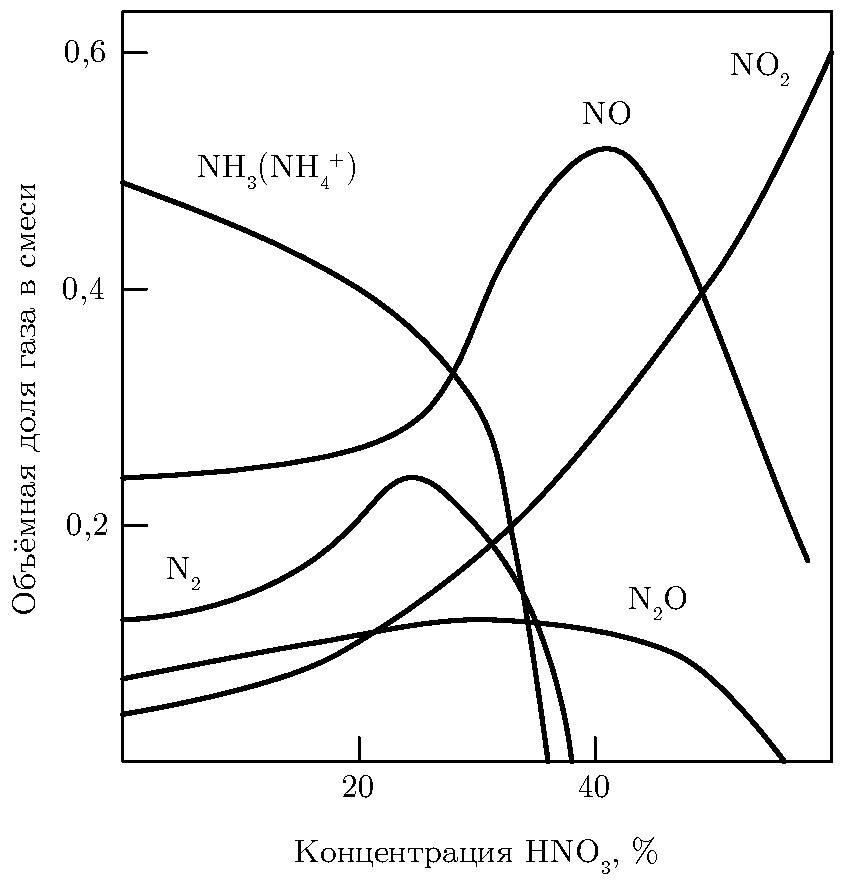
\includegraphics[width=8cm]{figs/writing_redox_equations/products_of_the_reaction_of_iron_with_nitric_acid.pdf}
    \caption{Продукты, образующиеся при реакции железа с азотной кислотой.}
    \label{fig:products_of_the_reaction_of_iron_with_nitric_acid}
\end{figure}

Образование \ce{NO2} (бурый газ) происходит при взаимодействии концентрированной кислоты и малоактивных металлов (\ce{Cu}, \ce{Ag}, \ce{Hg} и пр.):

\reaction*{Cu + 4HNO3_{\text{(конц.)}} -> Cu(NO3)2 + 2NO2 (^) + 2H2O{.}}

Образование \ce{NO} (бесцветный газ) типично для разбавленной кислоты и металлов низкой и средней активности (\ce{Cu}, \ce{Fe}, \ce{Ni}):

\reaction*{Fe + 4HNO3_{\text{(разб.)}} -> Fe(NO3)3 + NO (^) + 2H2O{.}}

Образование \ce{N2O}\footnote{Бесцветный газ, тривиальное название~--- <<веселящий газ>>.} наблюдается при взаимодействии разбавленной \ce{HNO3} с активными металлами (\ce{Zn}, \ce{Mg}, \ce{Al}):

\reaction*{4Zn + 10HNO3_{\text{(разб.)}} -> 4Zn(NO3)2 + N2O (^) + 5H2O{.}}

Образование \ce{NH3}/\ce{NH4^+} характерно для очень разбавленной кислоты и самых активных металлов (\ce{Ca}, \ce{Mg}):

\reaction*{4Mg + 10HNO3_{\text{(оч. разб.)}} -> 4Mg(NO3)2 + NH4NO3 + 3H2O{.}}

Итак, чем сильнее восстановитель и чем более разбавлена азотная кислота, тем глубже происходит восстановление. Нагревание обычно тоже увеличивает глубину восстановления (рис.~\ref{fig:effect_of_conditions_on_the_reduction_of_nitric_acid}).

\begin{figure}[htbp]
    \centering
    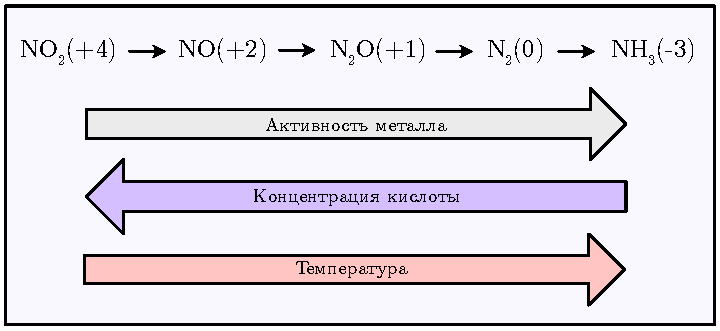
\includegraphics[width=10cm]{figs/writing_redox_equations/effect_of_conditions_on_the_reduction_of_nitric_acid.pdf}
    \caption{Влияние условий реакции на восстановление азотной кислоты.}
    \label{fig:effect_of_conditions_on_the_reduction_of_nitric_acid}
\end{figure}

Все варианты взаимодействия азотной кислоты разной концентрации с различными химическими элементами поначалу запомнить трудно. Поэтому в качестве справочной информации вы можете воспользоваться таблицей продуктов реакции элементов в периодической системе с азотной кислотой из приложения~\ref{appendix:reaction_of_chemical_elements_with_nitric_acid}. 

\subsection*{Влияние температуры на ход ОВР}

С ростом температуры усиливается диспропорционирование~--- разница в степенях окисления в продуктах растёт. Вот наглядный пример (табл.~\ref{tab:reaction_of_chlorine_with_alkali}):

\begin{table}[htbp]
    \small
    \caption{Реакция хлора со щёлочью.}
    \label{tab:reaction_of_chlorine_with_alkali}
    \begin{tabularx}{\textwidth}{
        >{\hsize=0.7\hsize}Y
        >{\hsize=1.3\hsize}Y
        }
        \hline
        \rowcolor{green!5}
        Условия & Реакция \\
        \hline
        С холодной щёлочью &  \ce{Cl2 + 2NaOH -> NaClO + NaCl + H2O} \\
        С горячей щёлочью & \ce{3Cl2 + 6NaOH -> NaClO3 + 5NaCl + 3H2O} \\
        \hline
    \end{tabularx}
\end{table}

\subsection*{Влияние катализатора на ход ОВР}

Без катализатора реакция окисления тиосульфата натрия перекисью водорода происходит с образованием тетратионата натрия:

\reaction*{2Na2S2O3 + H2O2 -> Na2S4O6 + 2NaOH{.}}

Но в присутствии \ce{H2MoO4} реакция протекает по-другому:

\reaction*{Na2S2O3 + 4H2O2 -> Na2SO4 + H2SO4 + 3H2O{.}}

Теперь давайте рассмотрим примеры решения задач.

\begin{example}{}{ex:writing_redox_equations1}
    \begin{condition}
        Допишите уравнение окислительно-восстановительной реакции и расставьте в нём коэффициенты методом электронного баланса:
        \reaction*{KMnO4 + KOH + K2SO3 ->{.}}
    \end{condition}

    \medskip

    \textit{Решение.} Определим продукты реакции. Для этого найдём элементы, являющиеся окислителем и восстановителем. Марганец находится в степени окисления +7 и может быть только окислителем. Поскольку среда щелочная, он должен восстанавливаться до степени окисления +6 с образованием манганат-анионов \ce{MnO4^{2-}}. Сера в степени окисления +4 проявляет свойства восстановителя, окисляясь до СО +6 с образованием сульфат-анионов. Составляем электронный баланс:
    \begin{align*}
        \overset{\textcolor{red}{+7}}{\ce{Mn}} + \ce{e- ->} \overset{\textcolor{red}{+6}}{\ce{Mn}} \quad &| 2 \\
        \overset{\textcolor{red}{+4}}{\ce{S}} - \ce{2e- ->} \overset{\textcolor{red}{+6}}{\ce{S}} \quad &| 1
    \end{align*}
    Также в продуктах реакции должна быть вода, чтобы сошёлся баланс по атомам водорода. Дописываем продукты реакции и расставляем коэффициенты:
    \reaction*{2KMnO4 + 2KOH + K2SO3 -> 2K2MnO4 + K2SO4 + H2O{.}}
\end{example}

\begin{example}{}{ex:writing_redox_equations2}
    \begin{condition}
        Допишите уравнение окислительно-восстановительной реакции и расставьте в нём коэффициенты методом полуреакций:
        \reaction*{K2Cr2O7 + H2SO4 + FeSO4 ->{.}}
    \end{condition}

    \medskip

    \textit{Решение.} Бихромат калия в кислой среде восстанавливается до солей трёхвалентного хрома:
    \reaction*{Cr2O7^{2-} + 14H+ + 6e- -> 2Cr^{3+} + 7H2O{.}}
    Сульфат железа (II) окисляется до сульфата железа (III):
    \reaction*{2FeSO4 + SO4^{2-} - 2e- -> Fe2(SO4)3{.}}
    Уравниваем электроны в полуреакциях и складываем уравнения:
    \begin{align*}
        \ce{Cr2O7^{2-} + 14H+ + 6e- -> 2Cr^{3+} + 7H2O} \quad &| 1 \\
        \ce{2FeSO4 + SO4^{2-} - 2e- -> Fe2(SO4)3} \quad &| 3
    \end{align*}
    \reaction*{Cr2O7^{2-} + 14H+ + 6FeSO4 + 3SO4^{2-} -> 2Cr^{3+} + 7H2O + 3Fe2(SO4)3{.}}
    Затем дополняем полученное уравнение до полного:
    \reaction*{K2Cr2O7 + 7H2SO4 + 6FeSO4 -> Cr2(SO4)3 + 3Fe2(SO4)3 + 7H2O + K2SO4{.}}
\end{example}

\begin{example}{}{ex:writing_redox_equations3}
    \begin{condition}
        Расставьте коэффициенты в уравнении:
        \reaction*{AsF3 + As2O3 + F2 -> As(O)F3{.}}
    \end{condition}

    \medskip

    \textit{Решение.} В этом уравнении \emph{два восстановителя}~--- мышьяк в степени окисления +3 в оксиде и в степени окисления +3 во фториде. И тот и другой окисляются до степени окисления +5 в оксофториде. Поскольку для обоих восстановителей протекает одна и та же реакция окисления, мы можем объединить уравнения окисления для обоих атомов мышьяка:
    \begin{align*}
        \overset{\textcolor{red}{+3}}{\ce{As}} - \ce{2e- ->} \overset{\textcolor{red}{+5}}{\ce{As}} \quad &| 1 \\
        \overset{\textcolor{red}{0}}{\ce{F2}} + \ce{2e- ->} 2\overset{\textcolor{red}{-1}}{\ce{F}} \quad &| 1
    \end{align*}
    Одна молекула фтора окисляет один атом мышьяка. Поскольку в левой части уравнения реакции три атома мышьяка, ставим коэффициент 3 перед фтором и уравниваем правую часть:
    \reaction*{AsF3 + As2O3 + 3F2 -> 3As(O)F3{.}}
\end{example}

\begin{example}{}{ex:writing_redox_equations4}
    \begin{condition}
        Расставьте коэффициенты в уравнении:
        \reaction*{B4C + NaOH + H2O -> Na[B(OH)4] + H2 + C{.}}
    \end{condition}

    \medskip

    \textit{Решение.} Выясним, какие элементы меняют СО в этом уравнении. Вначале необходимо решить вопрос со степенями окисления в карбиде бора. Согласно таблице электроотрицательностей, бор имеет меньшую, чем углерод, электроотрицательность, поэтому в этом соединении он имеет степень окисления +1, а углерод –4. В ходе реакции и бор, и углерод окисляются: бор до степени окисления +3, углерод до степени окисления 0. Окислителем в данной реакции служит водород со степенью окисления +1, в ходе реакции он восстанавливается до степени окисления 0. Таким образом, это реакция с двумя восстановителями, \emph{находящимися в одном соединении}. Это важный момент, потому что в этом случае мы точно знаем, что соотношение коэффициентов при уравнениях окисления будет соответствовать соотношению атомов в молекуле карбида бора~--- 4/1:
    \begin{align*}
        \overset{\textcolor{red}{+1}}{\ce{B}} - \ce{2e- ->} \overset{\textcolor{red}{+3}}{\ce{B}} \quad &| 4 \\
        \overset{\textcolor{red}{-4}}{\ce{C}} - \ce{4e- ->} \overset{\textcolor{red}{0}}{\ce{C}} \quad &| 1 \\
        2\overset{\textcolor{red}{+1}}{\ce{H}} + \ce{2e- ->} \overset{\textcolor{red}{0}}{\ce{H2}} \quad &|
    \end{align*}
    Подсчитаем суммарное число электронов, участвующее в окислении: $2 \cdot 4 + 4 = 12$. Поэтому коэффициент при уравнении восстановления должен быть равен шести:
    \begin{align*}
        \overset{\textcolor{red}{+1}}{\ce{B}} - \ce{2e- ->} \overset{\textcolor{red}{+3}}{\ce{B}} \quad &| 4 \\
        \overset{\textcolor{red}{-4}}{\ce{C}} - \ce{4e- ->} \overset{\textcolor{red}{0}}{\ce{C}} \quad &| 1 \\
        2\overset{\textcolor{red}{+1}}{\ce{H}} + \ce{2e- ->} \overset{\textcolor{red}{0}}{\ce{H2}} \quad &| 6
    \end{align*}
    В данном случае количество электронов в процессах окисления и восстановления оказалось чётным числом. Если бы число электронов в процессе восстановления водорода оказалось нечётным, то необходимо было бы удвоить коэффициенты перед всеми уравнениями, однако соотношение между уравнениями окисления бора и углерода всё равно осталось бы 4/1.

    Подставляем коэффициент 6 перед водородом и расставляем оставшиеся коэффициенты:
    \reaction*{B4C + 4NaOH + 12H2O -> 4Na[B(OH)4] + 6H2 + C{.}}
\end{example}

\begin{example}{}{ex:writing_redox_equations5}
    \begin{condition}
        Методом электронного баланса найдите коэффициенты в уравнении реакции разложения тиосульфата натрия:
        \reaction*{Na2S2O3 -> Na2SO4 + Na2S + S{.}}
    \end{condition}

    \medskip

    \textit{Решение.} Это не внутримолекулярная ОВР, как может показаться, а реакция диспропорционирования. Чтобы это понять, необходимо правильно расставить степени окисления атомов в исходном тиосульфате. В этом случае нельзя использовать метод расчёта СО по брутто-формуле и необходимо использовать расчёт СО по структурной формуле (в литературе вы можете встретить и другие варианты расстановки внутренних связей в данном соединении).
    \begin{center}
        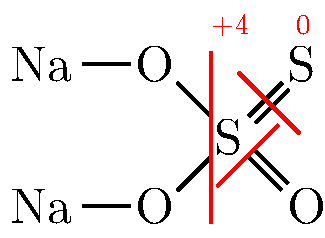
\includegraphics[width=2.2cm]{figs/writing_redox_equations/sodium_thiosulfate.pdf}
    \end{center}
    Поскольку в молекуле тиосульфата уже присутствует сера в степени окисления 0, очевидно, что она просто отщепляется от исходной молекулы. Записываем диспропорционирование серы в степени окисления +4 и расставляем коэффициенты:
    \begin{align*}
        \overset{\textcolor{red}{+4}}{\ce{S}} - \ce{2e- ->} \overset{\textcolor{red}{+6}}{\ce{S}} \quad &| 3 \\
        \overset{\textcolor{red}{+4}}{\ce{S}} + \ce{6e- ->} \overset{\textcolor{red}{-2}}{\ce{S}} \quad &| 1
    \end{align*}
    \reaction*{4Na2S2O3 -> 3Na2SO4 + Na2S + 4S{.}}
\end{example}

\begin{example}{}{ex:writing_redox_equations6}
    \begin{condition}
        Расставьте коэффициенты в уравнении:
        \reaction*{P2I4 + P4 + H2O -> PH4I + H3PO4{.}}
    \end{condition}

    \medskip

    \textit{Решение.} Вначале пытаемся определить окислитель и восстановитель и составляем электронный баланс:
    \begin{align*}
        2\overset{\textcolor{red}{+2}}{\ce{P}} + \ce{10e- ->} 2\overset{\textcolor{red}{-3}}{\ce{P}} \quad &| 2 \\
        4\overset{\textcolor{red}{0}}{\ce{P}} - \ce{20e- ->} 4\overset{\textcolor{red}{+5}}{\ce{P}} \quad &| 1
    \end{align*}
    Подставив эти коэффициенты в уравнения реакций, мы обнаружим, что количества атомов иода и водорода не уравниваются. Наличие <<лишних>> атомов иода и водорода означает, что процесс(ы) окисления или восстановления протекают не так, как мы написали, иначе ОВР уравнялась бы. Это означает, что в реакции одновременно происходит либо два разных процесса окисления, либо два разных процесса восстановления. Поскольку реагентов, содержащих фосфор, всего два, один из них является одновременно и окислителем, и восстановителем, т.~е. диспропорционирует. В уравнении реакции есть фосфор в степенях окисления +2 и 0. Фосфору в степени окисления 0 проще диспропорционировать, поскольку забирать электроны у атома со степенью окисления +2 сложнее. Поэтому записываем баланс не из двух реакций, а из трёх:
    \begin{align*}
        2\overset{\textcolor{red}{+2}}{\ce{P}} + \ce{10e- ->} 2\overset{\textcolor{red}{-3}}{\ce{P}} \quad &| x \\
        4\overset{\textcolor{red}{0}}{\ce{P}} + \ce{12e- ->} 4\overset{\textcolor{red}{-3}}{\ce{P}} \quad &| y \\
        4\overset{\textcolor{red}{0}}{\ce{P}} - \ce{20e- ->} 4\overset{\textcolor{red}{+5}}{\ce{P}} \quad &| z
    \end{align*}
    Баланс по электронам будет выполнен при условии $10x + 12y = 20z$ или $5x + 6y = 10z$. Коэффициенты находим методом подбора: $x = 10$, $y = 5$, $z = 8$, и окончательно уравниваем ОВР:
    \reaction*{10P2I4 + 13P4 + 128H2O -> 40PH4I + 32H3PO4{.}}
\end{example}

\begin{problem}{}{writing_redox_equations1}
    Расставьте коэффициенты в уравнениях следующих ОВР: \\
    а) \ce{FeO + Al ->[\qty{500}{\degreeCelsius}] Al2O3 + Fe{;}} \\
    б) \ce{KClO4 + Al ->[\qty{700}{\degreeCelsius}] KCl + Al2O3{;}} \\
    в) \ce{K2CrO4 + Zr ->[\qty{800}{\degreeCelsius}] K + Zr(CrO4)2{;}} \\
    г) \ce{KOH + K ->[\qty{450}{\degreeCelsius}] K2O + H2{.}}
    \begin{sol}{\ref{prob:writing_redox_equations1}}
        а) \ce{3FeO + 2Al ->[\qty{500}{\degreeCelsius}] Al2O3 + 3Fe{;}}
        \begin{align*}
            \overset{\textcolor{red}{+2}}{\ce{Fe}} + \ce{2e- ->} \overset{\textcolor{red}{0}}{\ce{Fe}} \quad &| 3 \\
            \overset{\textcolor{red}{0}}{\ce{Al}} - \ce{3e- ->} \overset{\textcolor{red}{+3}}{\ce{Al}} \quad &| 2
        \end{align*}
        б) \ce{3KClO4 + 8Al ->[\qty{700}{\degreeCelsius}] 3KCl + 4Al2O3{;}}
        \begin{align*}
            \overset{\textcolor{red}{+7}}{\ce{Cl}} + \ce{8e- ->} \overset{\textcolor{red}{-1}}{\ce{Cl}} \quad &| 3 \\
            \overset{\textcolor{red}{0}}{\ce{Al}} - \ce{3e- ->} \overset{\textcolor{red}{+3}}{\ce{Al}} \quad &| 8
        \end{align*}
        в) \ce{2K2CrO4 + Zr ->[\qty{800}{\degreeCelsius}] 4K + Zr(CrO4)2{;}}
        \begin{align*}
            \overset{\textcolor{red}{+1}}{\ce{K}} + \ce{e- ->} \overset{\textcolor{red}{0}}{\ce{K}} \quad &| 4 \\
            \overset{\textcolor{red}{0}}{\ce{Zr}} - \ce{4e- ->} \overset{\textcolor{red}{+4}}{\ce{Zr}} \quad &| 1
        \end{align*}
        г) \ce{2KOH + 2K ->[\qty{450}{\degreeCelsius}] 2K2O + H2{.}}
        \begin{align*}
            2\overset{\textcolor{red}{+1}}{\ce{H}} + \ce{2e- ->} \overset{\textcolor{red}{0}}{\ce{H2}} \quad &| 1 \\
            \overset{\textcolor{red}{0}}{\ce{K}} - \ce{e- ->} \overset{\textcolor{red}{+1}}{\ce{K}} \quad &| 2
        \end{align*}
    \end{sol}
\end{problem}

\begin{problem}{}{writing_redox_equations2}
    Допишите продукты в следующих уравнениях ОВР с участием перманганата калия и расставьте коэффициенты: \\
    а) \ce{KMnO4 + H2SO4_{(\text{разб.})} + KNO2 ->{;}} \\
    б) \ce{KMnO4 + H2SO4_{(\text{разб.})} + H2O2 ->{;}} \\
    в) \ce{KMnO4 + KOH_{(\text{конц.})} + K2SO3 ->{;}} \\
    г) \ce{KMnO4 + H2O + K2SO3_{(\text{конц.})} ->{.}}
    \begin{sol}{\ref{prob:writing_redox_equations2}}
        а) \ce{2KMnO4 + 3H2SO4_{(\text{разб.})} + 5KNO2 -> 2MnSO4 + 5KNO3 + K2SO4 + 3H2O{;}}
        \begin{align*}
            \overset{\textcolor{red}{+7}}{\ce{Mn}} + \ce{5e- ->} \overset{\textcolor{red}{+2}}{\ce{Mn}} \quad &| 2 \\
            \overset{\textcolor{red}{+3}}{\ce{N}} - \ce{2e- ->} \overset{\textcolor{red}{+5}}{\ce{N}} \quad &| 5
        \end{align*}
        б) \ce{2KMnO4 + 3H2SO4_{(\text{разб.})} + 5H2O2 -> 2MnSO4 + 5O2 (^) + 8H2O + K2SO4{;}}
        \begin{align*}
            \overset{\textcolor{red}{+7}}{\ce{Mn}} + \ce{5e- ->} \overset{\textcolor{red}{+2}}{\ce{Mn}} \quad &| 2 \\
            2\overset{\textcolor{red}{-1}}{\ce{O}} - \ce{2e- ->} \overset{\textcolor{red}{0}}{\ce{O2}} \quad &| 5
        \end{align*}
        в) \ce{2KMnO4 + 2KOH_{(\text{конц.})} + K2SO3 -> 2K2MnO4 + K2SO4 + H2O{;}}
        \begin{align*}
            \overset{\textcolor{red}{+7}}{\ce{Mn}} + \ce{e- ->} \overset{\textcolor{red}{+6}}{\ce{Mn}} \quad &| 2 \\
            \overset{\textcolor{red}{+4}}{\ce{S}} - \ce{2e- ->} \overset{\textcolor{red}{+6}}{\ce{S}} \quad &| 1
        \end{align*}
        г) \ce{2KMnO4 + H2O + 3K2SO3_{(\text{конц.})} -> 2MnO2 (v) + 3K2SO4 + 2KOH{.}}
        \begin{align*}
            \overset{\textcolor{red}{+7}}{\ce{Mn}} + \ce{3e- ->} \overset{\textcolor{red}{+4}}{\ce{Mn}} \quad &| 2 \\
            \overset{\textcolor{red}{+4}}{\ce{S}} - \ce{2e- ->} \overset{\textcolor{red}{+6}}{\ce{S}} \quad &| 3
        \end{align*}
    \end{sol}
\end{problem}

\clearpage